\chapter{Programm Launch}
\label{chap:programlaunch}
In diesem Kapitel wird beschrieben, wie das kompilierte uForth-Programm aus der Entwicklungsumgebung gestartet werden kann und was dafür implementiert wurde.

\section{Launch}

In Eclipse wird zwischen zwei Launch-Möglichkeiten unterschieden. In den nächsten Kapiteln werden die zwei Launch-Möglichkeiten erklärt.

\begin{figure}[H]
	\centering
		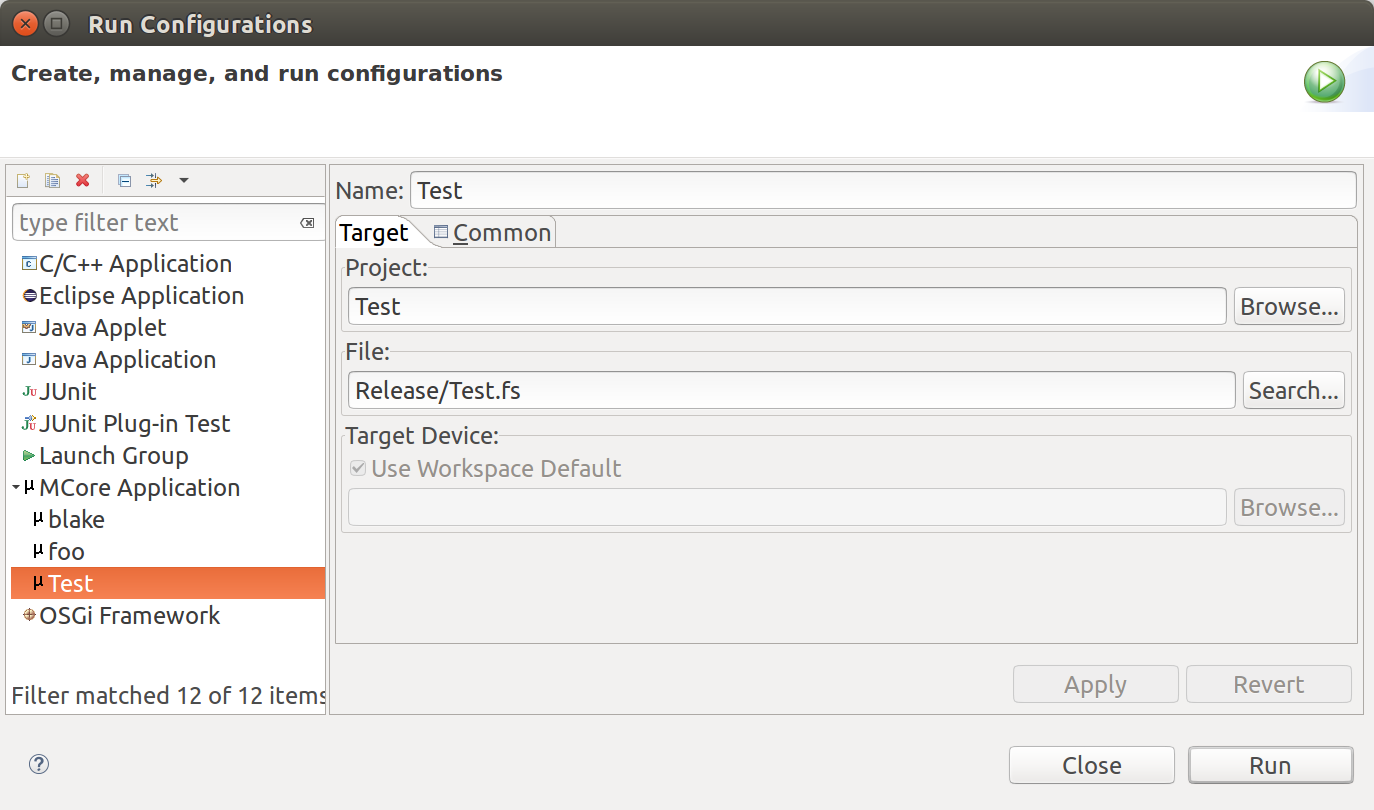
\includegraphics[scale=0.3]{launch/run.png}
		\caption{Der Launch Configuration Dialog. In diesem Dialog kann eine neue MCore Launch-Konfiguration erstellt werden. Um eine gültige Konfiguration zu erstellen, muss das Projekt und das Forth File, das gestartet werden soll, angegeben werden.}
		\captionsetup{margin=0cm,font={footnotesize}}
		\label{fig:run}
\end{figure}

\newpage
\subsection{Run}

Mit der Run-Konfiguration wird zuerst der Loader in den Forth Workspace kopiert, der in den Umgebungsvariablen definiert sein muss. Danach wird der Forth-Prozess gestartet und der Umbilical Port mittels \verb!Umbilical: /dev/ttyUSBX! gesetzt. Der Umbilical Port und der Loader müssen in der MCore Preference Page gesetzt werden (siehe Kapitel \nameref{chap:settings}). Falls der Umbilical Port ungültig ist, erscheint beim starten des Programms eine Fehlermeldung.

\begin{figure}[H]
	\centering
		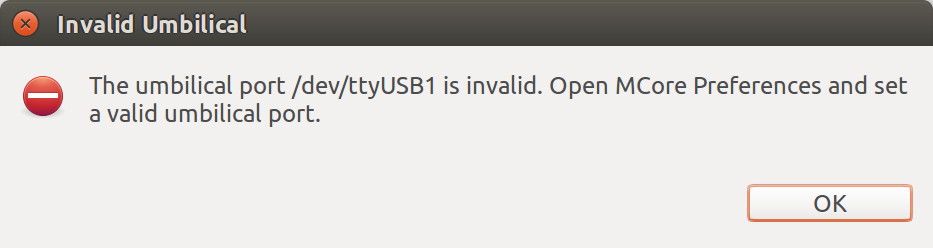
\includegraphics[scale=0.4]{launch/invalidumbilical.png}
		\caption{Dialog, der erscheint, wenn ein Programm gestartet wird und der Umbilical Port ungültig ist. Der Port kann in der MCore Preference Page geändert werden.}
		\captionsetup{margin=0cm,font={footnotesize}}
		\label{fig:invalidumbilical}
\end{figure}

\subsection{Debug}

In der Debug-Konfiguration werden zusätzlich alle Funktionen des gestarteten Forth Files disassembliert. Dies wird gemacht, damit der Debugger die Funktionen in einem File anzeigen kann. Es kann nicht der vom Compiler generierte Code genommen werden, da der Forth Cross-Compiler noch Optimierungen am Code vornimmt.

